\setlength{\columnsep}{3pt}
\begin{flushleft}
	\bigskip
	\begin{itemize}

		\begin{figure}[h!]
			\centering
			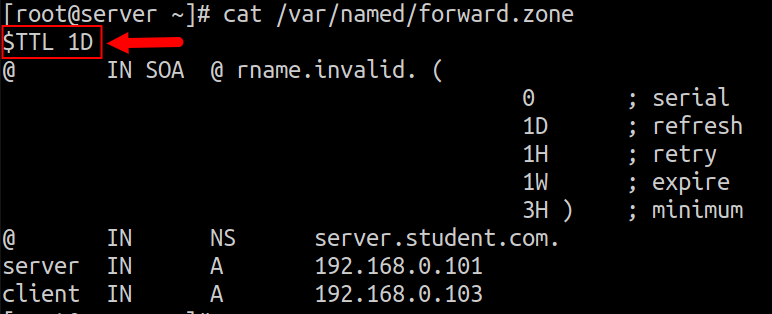
\includegraphics[scale=.4]{content/chapter3/images/zone1.png}
		\end{figure}
		\item \$TTL – DNS TTL (time to live) is a setting that tells the DNS resolver how long to cache a query before requesting a new one.

		\newpage
		\begin{figure}[h!]
			\centering
			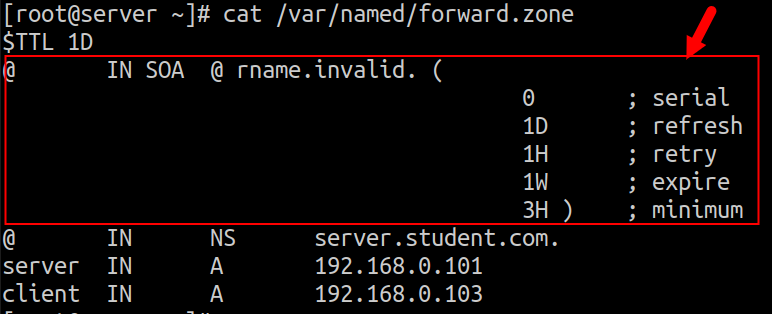
\includegraphics[scale=.4]{content/chapter3/images/zone2.png}
		\end{figure}
		\begin{tcolorbox}[breakable,notitle,boxrule=1pt,colback=pink,colframe=pink]
			\color{black}
			\fontdimen2\font=2em
			Syntax: 

			\newline
			@   IN  SOA  @  hostmaster-email (
			\newline
			serial-number
			\newline
			time-to-refresh
			\newline
			time-to-retry
			\newline
			time-to-expire
			\newline
			minimum-TTL)
			\fontdimen2\font=4pt
		\end{tcolorbox}	
		
		\begin{itemize}
			\item @ means domain-name
			\item IN: Stands for Internet
			\item SOA: The DNS ‘start of authority’ (SOA) record stores important information about a domain or zone such as the email address of the administrator, when the domain was last updated, and how long the server should wait between refreshes.
			\item 
			
		\end{itemize}
		
		\newpage
		\begin{figure}[h!]
			\centering
			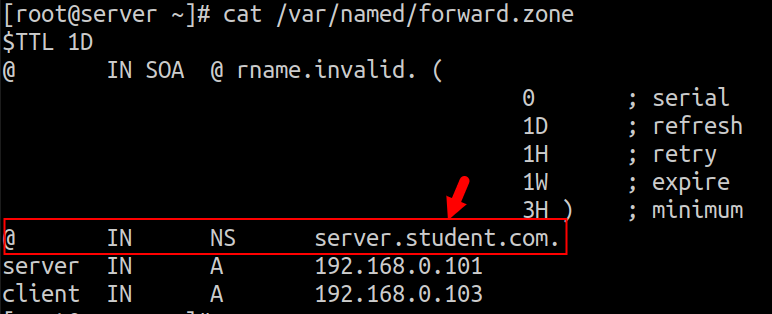
\includegraphics[scale=.4]{content/chapter3/images/zone3.png}
		\end{figure}
		\begin{tcolorbox}[breakable,notitle,boxrule=1pt,colback=pink,colframe=pink]
			\color{black}
			\fontdimen2\font=2em
			Syntax: 
			\newline
			\color{blue}
			@   IN  SOA  @  hostmaster-email (
			\newline
			serial-number
			\newline
			time-to-refresh
			\newline
			time-to-retry
			\newline
			time-to-expire
			\newline
			minimum-TTL)
			\fontdimen2\font=4pt
		\end{tcolorbox}	
		\begin{itemize}
			\item The DNS ‘start of authority’ (SOA) record stores important information about a domain or zone such as the email address of the administrator, when the domain was last updated, and how long the server should wait between refreshes.
		\end{itemize}			
		
	\end{itemize}
\end{flushleft}

\newpage





